\hypertarget{framever_8c}{
\section{framever.c File Reference}
\label{framever_8c}\index{framever.c@{framever.c}}
}
{\tt \#include $<$stdlib.h$>$}\par
{\tt \#include $<$stdio.h$>$}\par
{\tt \#include $<$string.h$>$}\par
{\tt \#include $<$unistd.h$>$}\par
{\tt \#include \char`\"{}dcsc\-Msg\-Buffer\-Interface.h\char`\"{}}\par
{\tt \#include \char`\"{}framever.h\char`\"{}}\par
{\tt \#include $<$sys/stat.h$>$}\par
{\tt \#include $<$sys/time.h$>$}\par


Include dependency graph for framever.c:\begin{figure}[H]
\begin{center}
\leavevmode
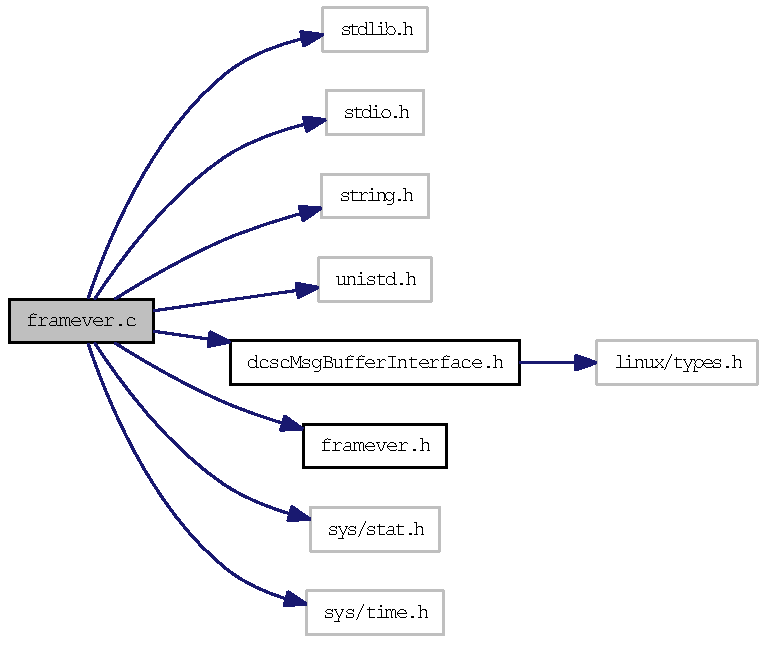
\includegraphics[width=202pt]{framever_8c__incl}
\end{center}
\end{figure}
\subsection*{Functions}
\begin{CompactItemize}
\item 
int \hyperlink{framever_8c_3c04138a5bfe5d72780bb7e82a18e627}{main} (int argc, char $\ast$$\ast$argv)
\item 
int \hyperlink{framever_8c_6452a9d7c9fcabeb40bb5d8495300090}{step} ()
\begin{CompactList}\small\item\em do the step-by-step frame verification \item\end{CompactList}\item 
\_\-\_\-u32 \hyperlink{framever_8c_5f1e2c849d7d370196a9a235300ed810}{get\-Errorcounter\-Reg} ()
\begin{CompactList}\small\item\em reads out the R\_\-Err\-Cnt register of the Xilinx which holds the number of errors found by readback and verification of Xilinx configuration memory \item\end{CompactList}\item 
\_\-\_\-u32 \hyperlink{framever_8c_27f551c32cffbe0aafb55212b34c09f4}{get\-Last\-Error\-Framenumber} ()
\begin{CompactList}\small\item\em reads out the RB\_\-Err\_\-Frame\-Number register of the Xilinx which holds the last frame number with an error as given by the sequence stored in the flash memory \item\end{CompactList}\item 
\_\-\_\-u32 \hyperlink{framever_8c_d5c190b1ed1cf08352c212a50559b2b4}{get\-Last\-Framenumber} ()
\begin{CompactList}\small\item\em reads out the RB\_\-Frame\-Number register of the Xilinx which holds the number of the last frame being verified as given by the sequence stored in the flash memory \item\end{CompactList}\item 
\_\-\_\-u32 \hyperlink{framever_8c_c45a0c5cc263cd2e94c6b392767c7f5b}{get\-Number\-Of\-Cycles} ()
\begin{CompactList}\small\item\em reads the RB\_\-num\-Of\-Cycles register of the Xilinx which holds the number of times a complete Frame by Frame readback of all frames has been done \item\end{CompactList}\item 
\_\-\_\-u32 \hyperlink{framever_8c_ac56165fccfc5df54af9983bef507775}{read\-Status\-Reg} ()
\begin{CompactList}\small\item\em reads the status register of the Xilinx \item\end{CompactList}\item 
\_\-\_\-u32 \hyperlink{framever_8c_fd9844f5942a7d95a2170dc4eda83cf6}{read\-Err\-Reg} ()
\begin{CompactList}\small\item\em reads the error register of the Xilinx \item\end{CompactList}\item 
int \hyperlink{framever_8c_3cd2524f3d82db41563298b30b223e9a}{clear\-Err\-Reg} ()
\begin{CompactList}\small\item\em clears the error register of the Xilinx \item\end{CompactList}\item 
int \hyperlink{framever_8c_05848de25ac2dbec233935058a1d24b4}{init} ()
\begin{CompactList}\small\item\em resets the controller, overwrites the flash cache memory and the selectmap memory, clears the status and error register. \item\end{CompactList}\item 
int \hyperlink{framever_8c_5b4325e5a0e8fa3ae1c169a04e3ded7c}{write\-Header\-To\-Logfile} ()
\begin{CompactList}\small\item\em Clears and opens the logfile and write a header to it, containing a timestamp. \item\end{CompactList}\item 
int \hyperlink{framever_8c_d4a2a88e7e0087ff1bbf6cbf8032aa15}{analyze16bit} (\_\-\_\-u16 bitfield)
\begin{CompactList}\small\item\em Takes 16 bits, counts and returns the occuring \char`\"{}1\char`\"{}s. \item\end{CompactList}\end{CompactItemize}


\subsection{Function Documentation}
\hypertarget{framever_8c_d4a2a88e7e0087ff1bbf6cbf8032aa15}{
\index{framever.c@{framever.c}!analyze16bit@{analyze16bit}}
\index{analyze16bit@{analyze16bit}!framever.c@{framever.c}}
\subsubsection[analyze16bit]{\setlength{\rightskip}{0pt plus 5cm}int analyze16bit (\_\-\_\-u16 {\em bitfield})}}
\label{framever_8c_d4a2a88e7e0087ff1bbf6cbf8032aa15}


Takes 16 bits, counts and returns the occuring \char`\"{}1\char`\"{}s. 

\begin{Desc}
\item[Parameters:]
\begin{description}
\item[{\em bitfield}]16 bits of which the \char`\"{}1\char`\"{}s should be counted \end{description}
\end{Desc}
\begin{Desc}
\item[Returns:]the number of ones in the 16 bit bitfield \end{Desc}


Definition at line 556 of file framever.c.

Referenced by main().\hypertarget{framever_8c_3cd2524f3d82db41563298b30b223e9a}{
\index{framever.c@{framever.c}!clearErrReg@{clearErrReg}}
\index{clearErrReg@{clearErrReg}!framever.c@{framever.c}}
\subsubsection[clearErrReg]{\setlength{\rightskip}{0pt plus 5cm}int clear\-Err\-Reg ()}}
\label{framever_8c_3cd2524f3d82db41563298b30b223e9a}


clears the error register of the Xilinx 

\begin{Desc}
\item[Returns:]-1 if something goes wrong \end{Desc}


Definition at line 463 of file framever.c.

References EXIT\_\-FAILURE, and rcu\-Single\-Write().

Referenced by main().

Here is the call graph for this function:\begin{figure}[H]
\begin{center}
\leavevmode
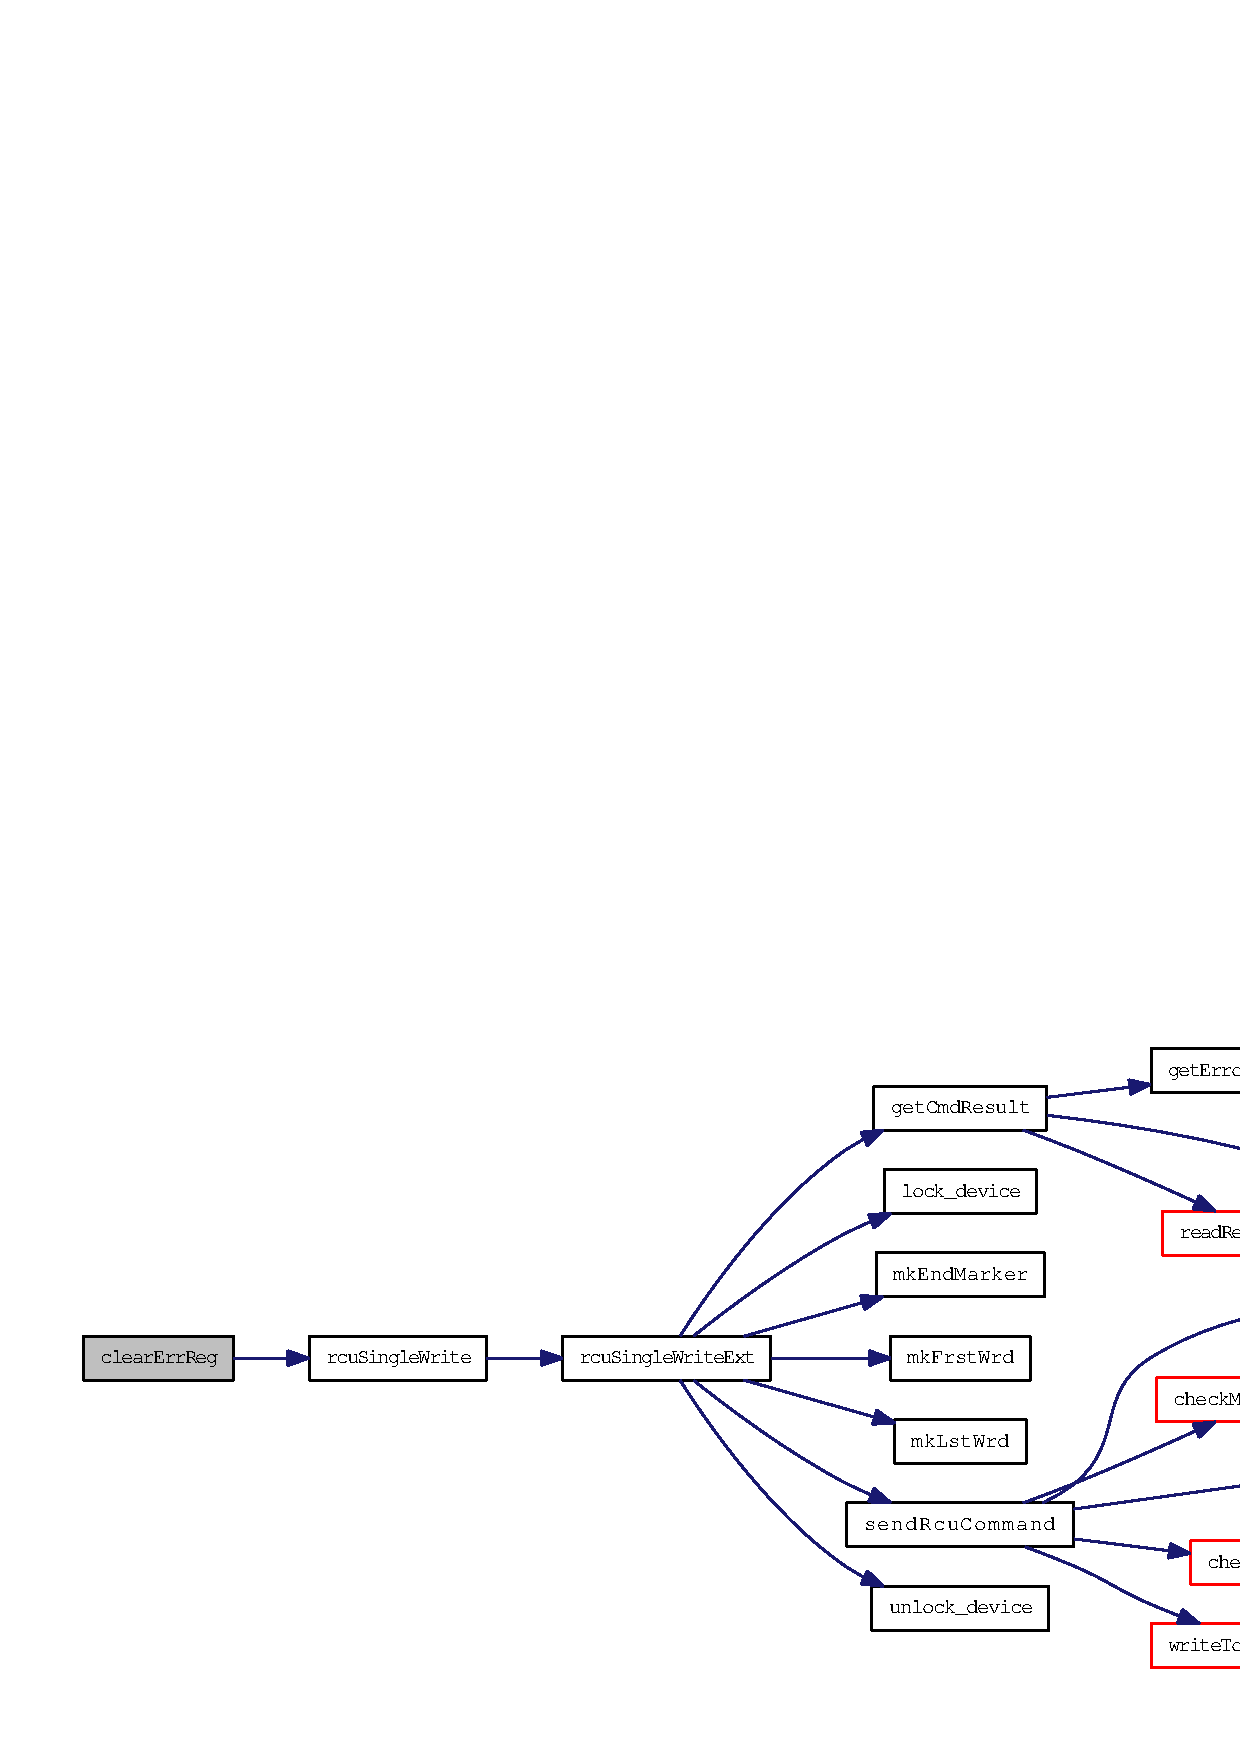
\includegraphics[width=403pt]{framever_8c_3cd2524f3d82db41563298b30b223e9a_cgraph}
\end{center}
\end{figure}
\hypertarget{framever_8c_5f1e2c849d7d370196a9a235300ed810}{
\index{framever.c@{framever.c}!getErrorcounterReg@{getErrorcounterReg}}
\index{getErrorcounterReg@{getErrorcounterReg}!framever.c@{framever.c}}
\subsubsection[getErrorcounterReg]{\setlength{\rightskip}{0pt plus 5cm}\_\-\_\-u32 get\-Errorcounter\-Reg ()}}
\label{framever_8c_5f1e2c849d7d370196a9a235300ed810}


reads out the R\_\-Err\-Cnt register of the Xilinx which holds the number of errors found by readback and verification of Xilinx configuration memory 

\begin{Desc}
\item[Returns:]the read data \end{Desc}


Definition at line 409 of file framever.c.

References EXIT\_\-FAILURE, and rcu\-Single\-Read().

Referenced by main().

Here is the call graph for this function:\begin{figure}[H]
\begin{center}
\leavevmode
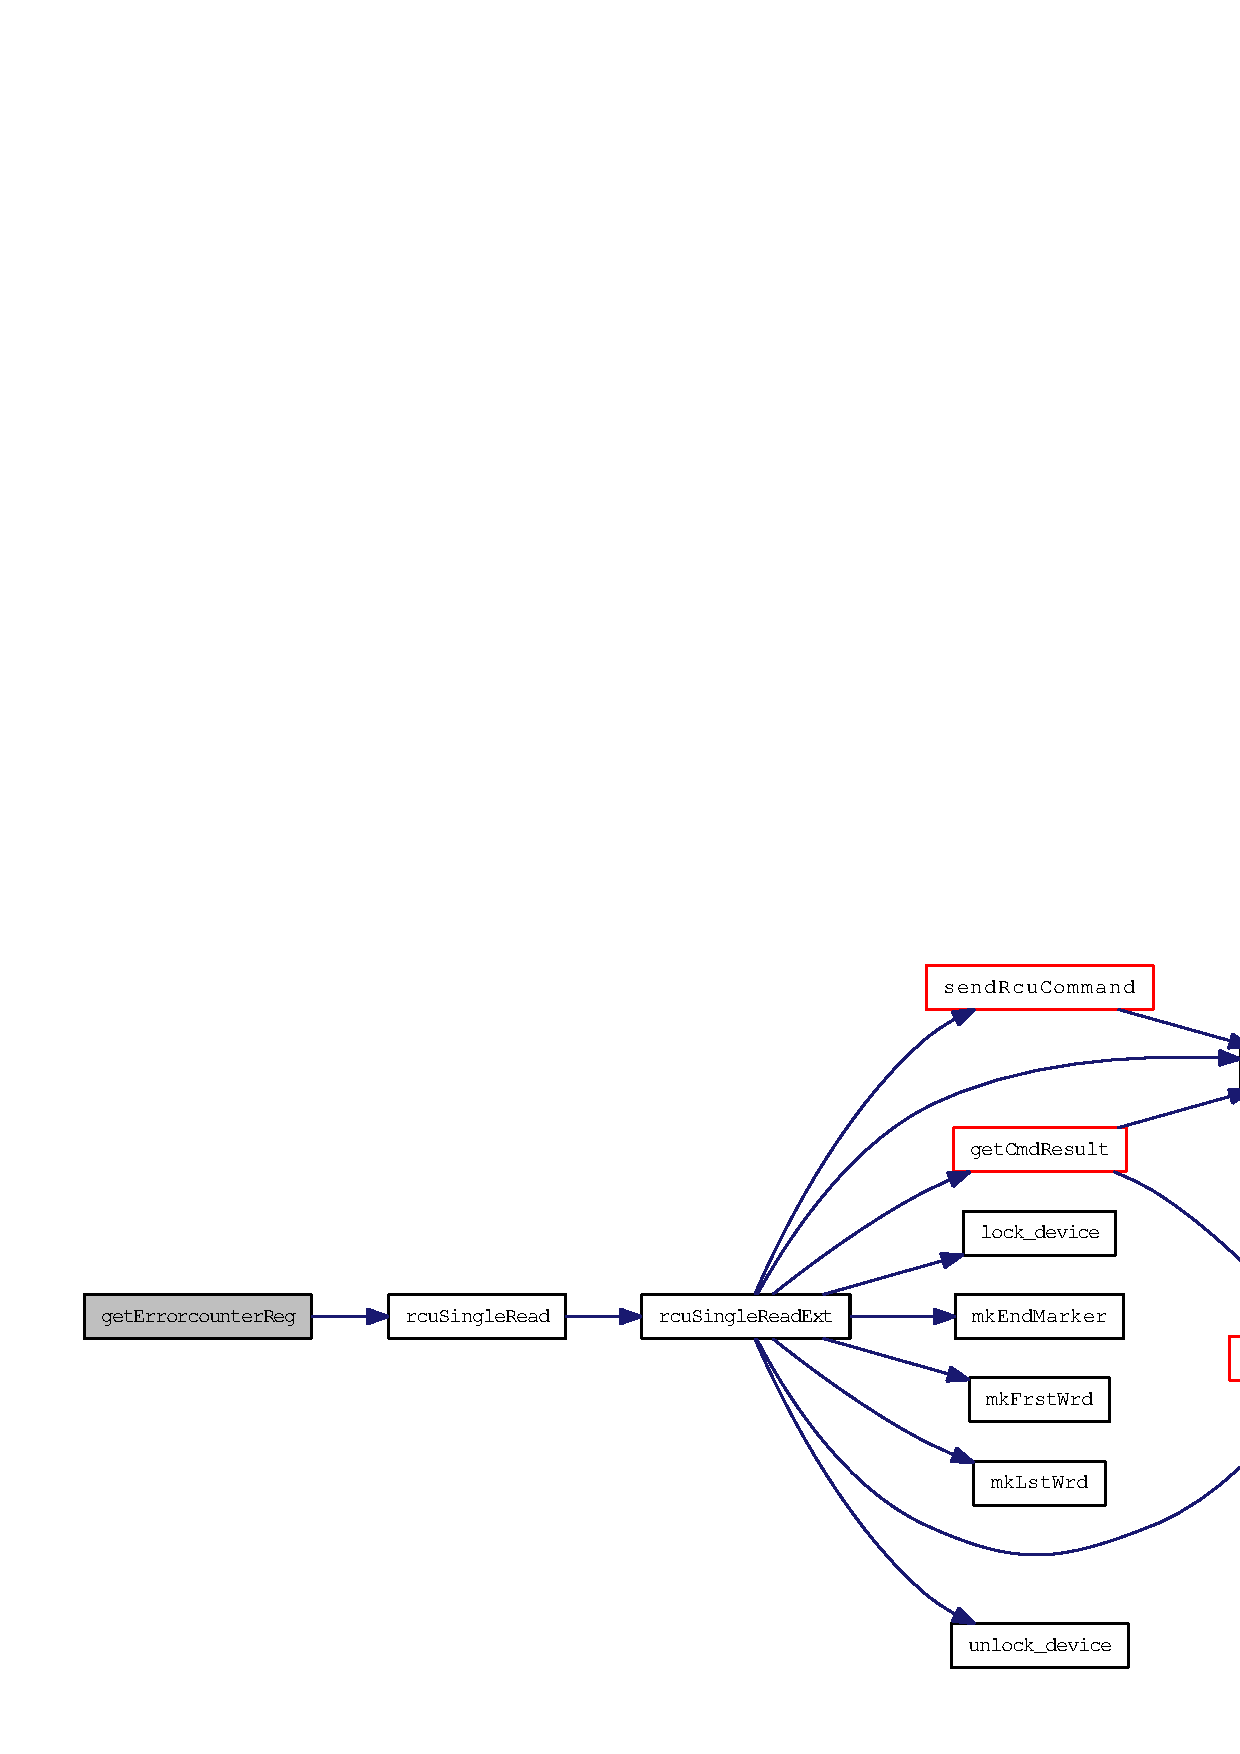
\includegraphics[width=345pt]{framever_8c_5f1e2c849d7d370196a9a235300ed810_cgraph}
\end{center}
\end{figure}
\hypertarget{framever_8c_27f551c32cffbe0aafb55212b34c09f4}{
\index{framever.c@{framever.c}!getLastErrorFramenumber@{getLastErrorFramenumber}}
\index{getLastErrorFramenumber@{getLastErrorFramenumber}!framever.c@{framever.c}}
\subsubsection[getLastErrorFramenumber]{\setlength{\rightskip}{0pt plus 5cm}\_\-\_\-u32 get\-Last\-Error\-Framenumber ()}}
\label{framever_8c_27f551c32cffbe0aafb55212b34c09f4}


reads out the RB\_\-Err\_\-Frame\-Number register of the Xilinx which holds the last frame number with an error as given by the sequence stored in the flash memory 

\begin{Desc}
\item[Returns:]returns the read data \end{Desc}


Definition at line 418 of file framever.c.

References EXIT\_\-FAILURE, and rcu\-Single\-Read().

Referenced by main().

Here is the call graph for this function:\begin{figure}[H]
\begin{center}
\leavevmode
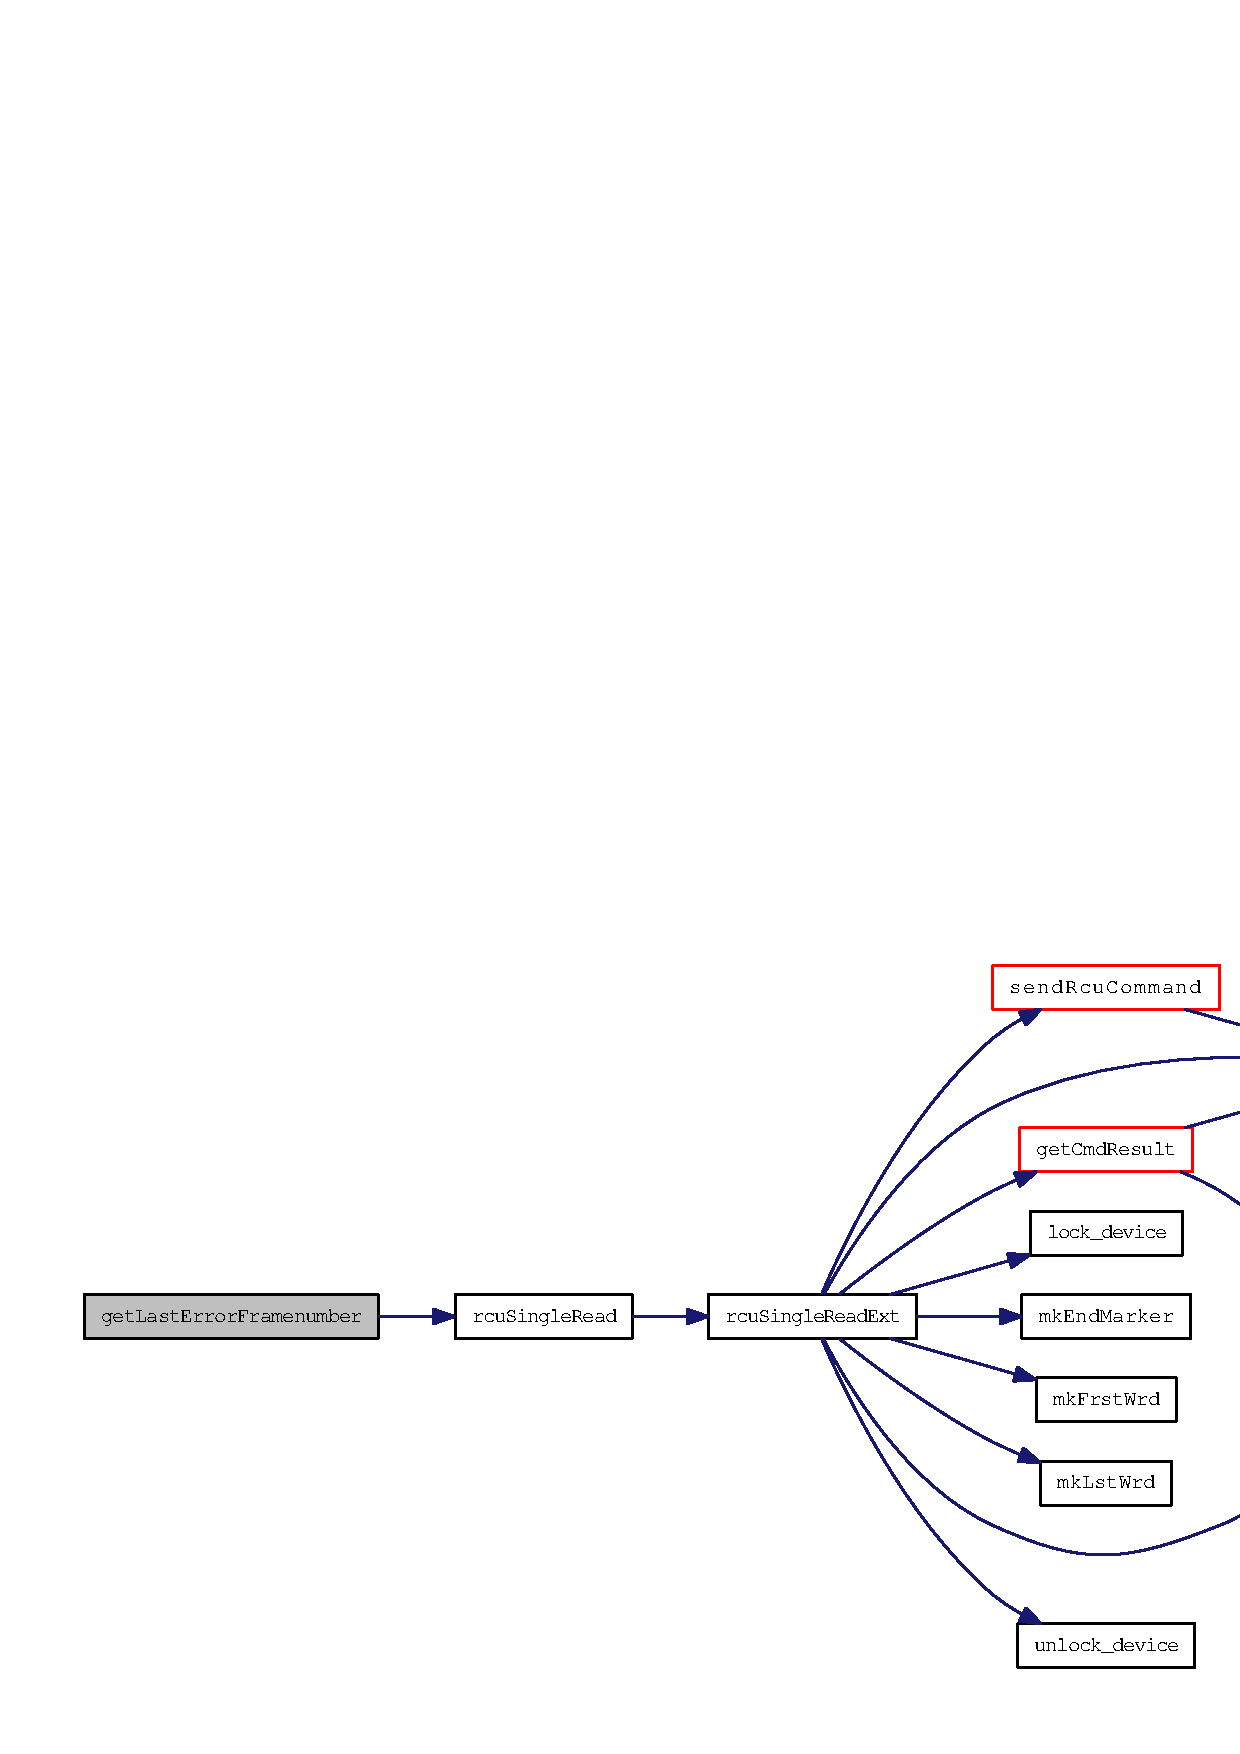
\includegraphics[width=361pt]{framever_8c_27f551c32cffbe0aafb55212b34c09f4_cgraph}
\end{center}
\end{figure}
\hypertarget{framever_8c_d5c190b1ed1cf08352c212a50559b2b4}{
\index{framever.c@{framever.c}!getLastFramenumber@{getLastFramenumber}}
\index{getLastFramenumber@{getLastFramenumber}!framever.c@{framever.c}}
\subsubsection[getLastFramenumber]{\setlength{\rightskip}{0pt plus 5cm}\_\-\_\-u32 get\-Last\-Framenumber ()}}
\label{framever_8c_d5c190b1ed1cf08352c212a50559b2b4}


reads out the RB\_\-Frame\-Number register of the Xilinx which holds the number of the last frame being verified as given by the sequence stored in the flash memory 

\begin{Desc}
\item[Returns:]returns the read data \end{Desc}


Definition at line 427 of file framever.c.

References EXIT\_\-FAILURE, and rcu\-Single\-Read().

Referenced by main().

Here is the call graph for this function:\begin{figure}[H]
\begin{center}
\leavevmode
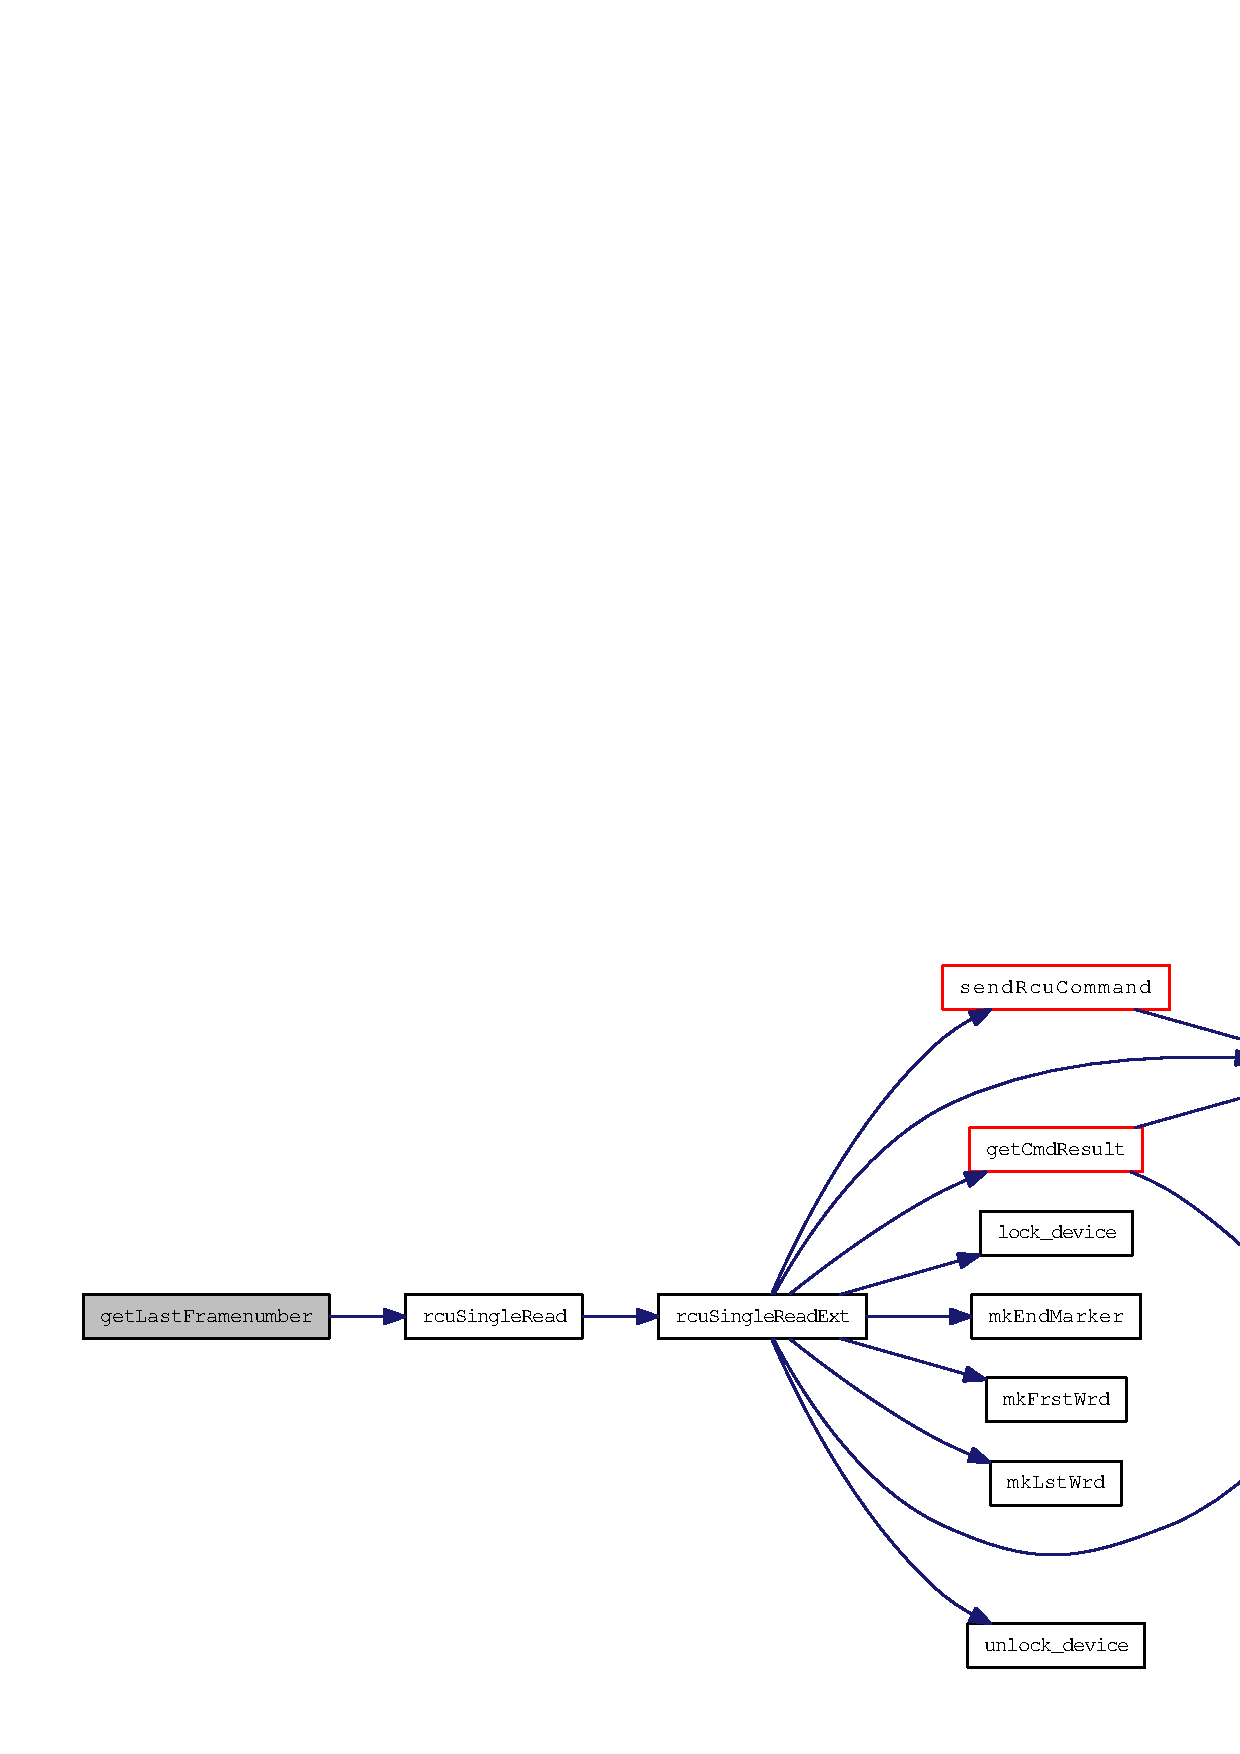
\includegraphics[width=349pt]{framever_8c_d5c190b1ed1cf08352c212a50559b2b4_cgraph}
\end{center}
\end{figure}
\hypertarget{framever_8c_c45a0c5cc263cd2e94c6b392767c7f5b}{
\index{framever.c@{framever.c}!getNumberOfCycles@{getNumberOfCycles}}
\index{getNumberOfCycles@{getNumberOfCycles}!framever.c@{framever.c}}
\subsubsection[getNumberOfCycles]{\setlength{\rightskip}{0pt plus 5cm}\_\-\_\-u32 get\-Number\-Of\-Cycles ()}}
\label{framever_8c_c45a0c5cc263cd2e94c6b392767c7f5b}


reads the RB\_\-num\-Of\-Cycles register of the Xilinx which holds the number of times a complete Frame by Frame readback of all frames has been done 

\begin{Desc}
\item[Returns:]returns the read data \end{Desc}


Definition at line 436 of file framever.c.

References EXIT\_\-FAILURE, and rcu\-Single\-Read().

Referenced by main().

Here is the call graph for this function:\begin{figure}[H]
\begin{center}
\leavevmode
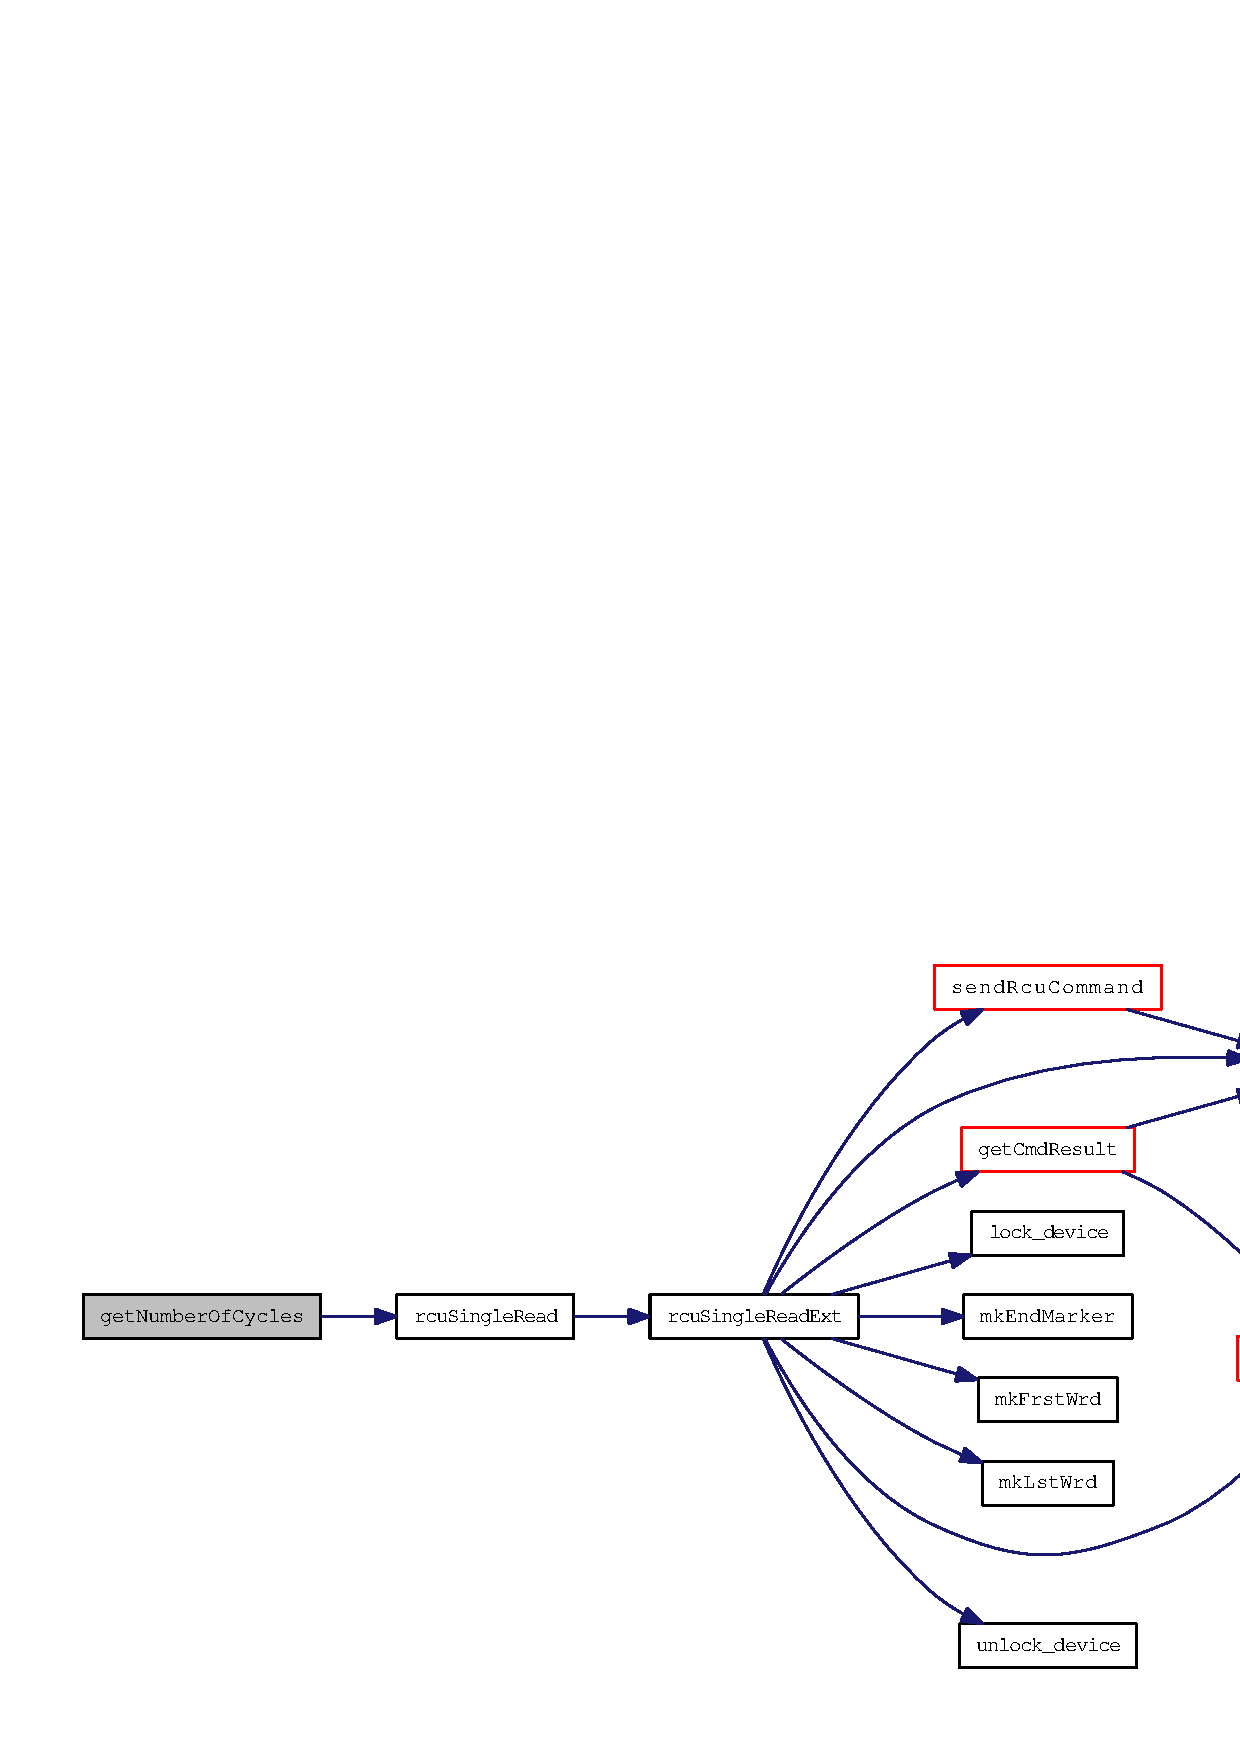
\includegraphics[width=347pt]{framever_8c_c45a0c5cc263cd2e94c6b392767c7f5b_cgraph}
\end{center}
\end{figure}
\hypertarget{framever_8c_05848de25ac2dbec233935058a1d24b4}{
\index{framever.c@{framever.c}!init@{init}}
\index{init@{init}!framever.c@{framever.c}}
\subsubsection[init]{\setlength{\rightskip}{0pt plus 5cm}int init ()}}
\label{framever_8c_05848de25ac2dbec233935058a1d24b4}


resets the controller, overwrites the flash cache memory and the selectmap memory, clears the status and error register. 

\begin{Desc}
\item[Returns:]an negative errorcode, 0 if successful \end{Desc}


Definition at line 474 of file framever.c.

References EXIT\_\-FAILURE, rcu\-Multiple\-Write(), and rcu\-Single\-Write().

Referenced by main().

Here is the call graph for this function:\begin{figure}[H]
\begin{center}
\leavevmode
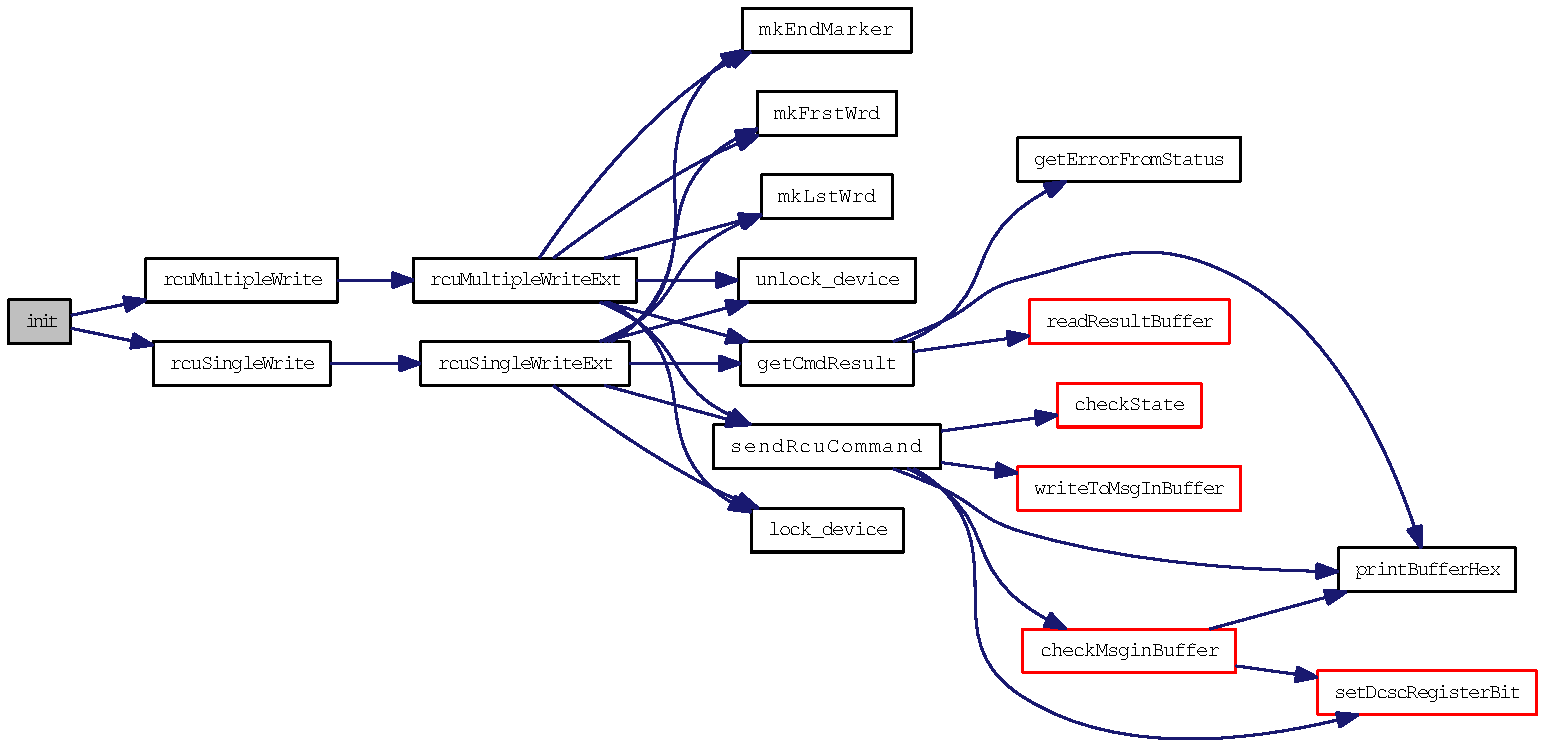
\includegraphics[width=389pt]{framever_8c_05848de25ac2dbec233935058a1d24b4_cgraph}
\end{center}
\end{figure}
\hypertarget{framever_8c_3c04138a5bfe5d72780bb7e82a18e627}{
\index{framever.c@{framever.c}!main@{main}}
\index{main@{main}!framever.c@{framever.c}}
\subsubsection[main]{\setlength{\rightskip}{0pt plus 5cm}int main (int {\em argc}, char $\ast$$\ast$ {\em argv})}}
\label{framever_8c_3c04138a5bfe5d72780bb7e82a18e627}




Definition at line 48 of file framever.c.

References analyze16bit(), clear\-Err\-Reg(), EXIT\_\-FAILURE, get\-Errorcounter\-Reg(), get\-Frame\-Address\-From\-Line(), get\-Last\-Error\-Framenumber(), get\-Last\-Framenumber(), get\-Linesnumber\-From\-File(), get\-Number\-Of\-Cycles(), init(), init\-Rcu\-Access(), rcu\-Multiple\-Read(), read\-Err\-Reg(), read\-Status\-Reg(), release\-Rcu\-Access(), step(), and write\-Header\-To\-Logfile().

Here is the call graph for this function:\begin{figure}[H]
\begin{center}
\leavevmode
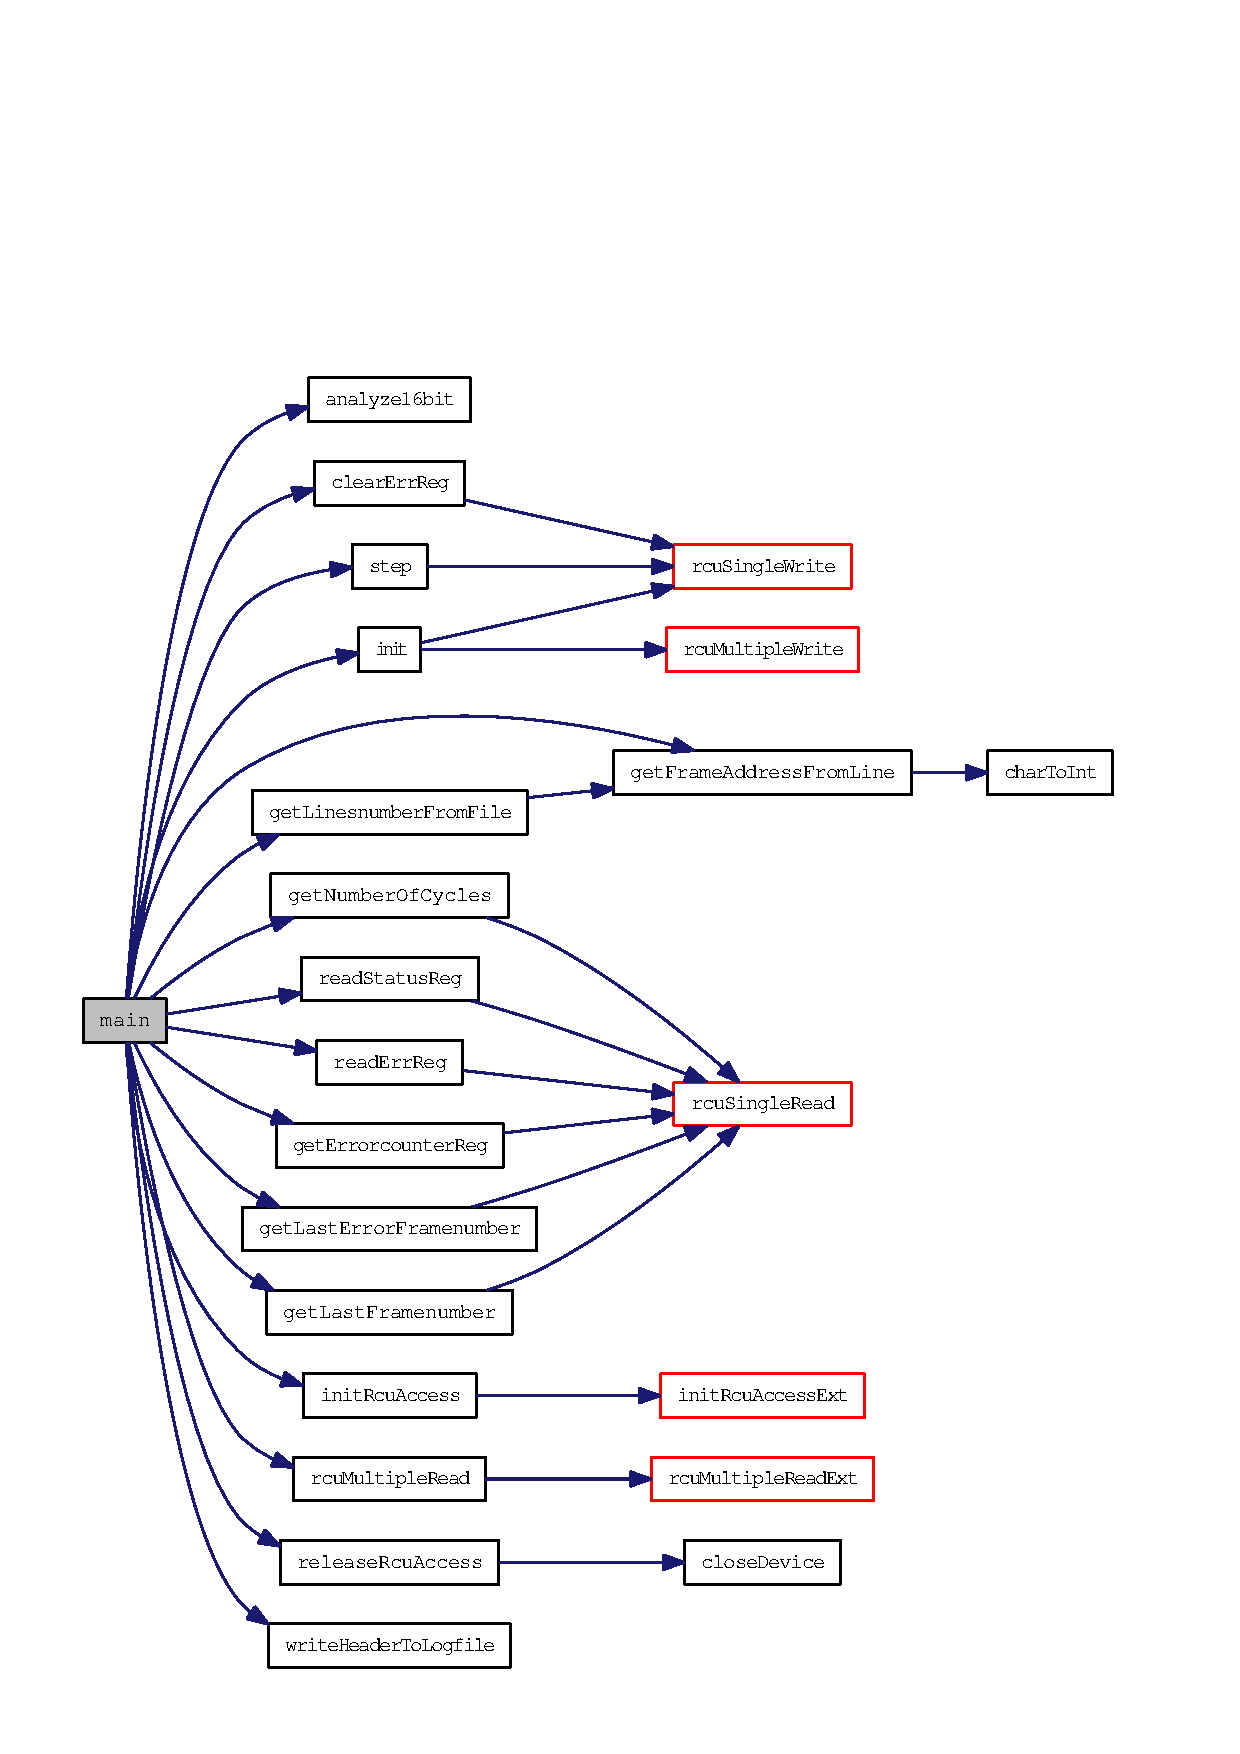
\includegraphics[width=269pt]{framever_8c_3c04138a5bfe5d72780bb7e82a18e627_cgraph}
\end{center}
\end{figure}
\hypertarget{framever_8c_fd9844f5942a7d95a2170dc4eda83cf6}{
\index{framever.c@{framever.c}!readErrReg@{readErrReg}}
\index{readErrReg@{readErrReg}!framever.c@{framever.c}}
\subsubsection[readErrReg]{\setlength{\rightskip}{0pt plus 5cm}\_\-\_\-u32 read\-Err\-Reg ()}}
\label{framever_8c_fd9844f5942a7d95a2170dc4eda83cf6}


reads the error register of the Xilinx 

\begin{Desc}
\item[Returns:]returns the read data \end{Desc}


Definition at line 454 of file framever.c.

References EXIT\_\-FAILURE, and rcu\-Single\-Read().

Referenced by main().

Here is the call graph for this function:\begin{figure}[H]
\begin{center}
\leavevmode
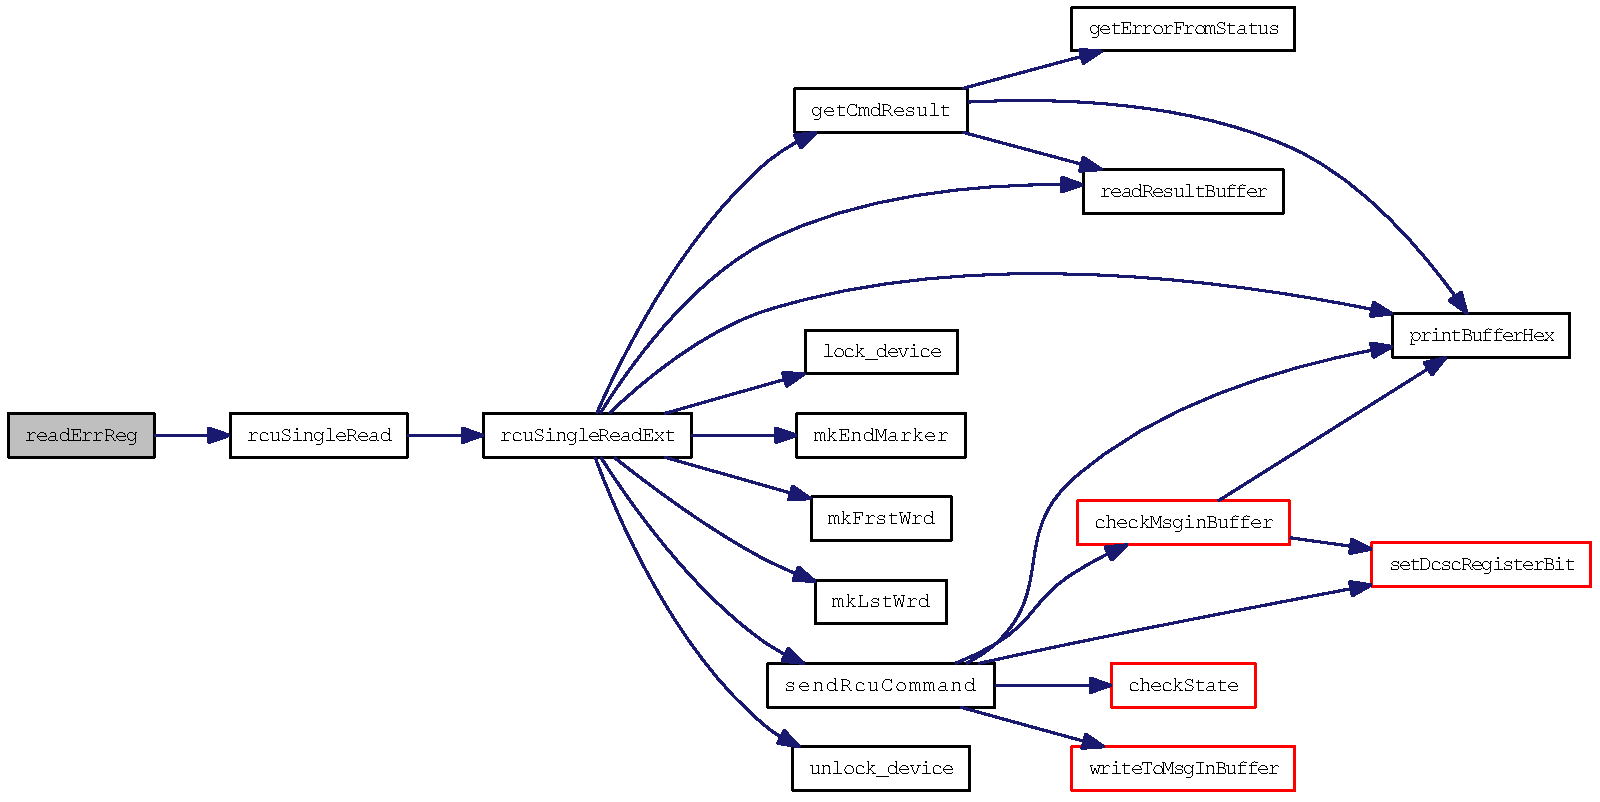
\includegraphics[width=402pt]{framever_8c_fd9844f5942a7d95a2170dc4eda83cf6_cgraph}
\end{center}
\end{figure}
\hypertarget{framever_8c_ac56165fccfc5df54af9983bef507775}{
\index{framever.c@{framever.c}!readStatusReg@{readStatusReg}}
\index{readStatusReg@{readStatusReg}!framever.c@{framever.c}}
\subsubsection[readStatusReg]{\setlength{\rightskip}{0pt plus 5cm}\_\-\_\-u32 read\-Status\-Reg ()}}
\label{framever_8c_ac56165fccfc5df54af9983bef507775}


reads the status register of the Xilinx 

\begin{Desc}
\item[Returns:]returns the read data \end{Desc}


Definition at line 445 of file framever.c.

References EXIT\_\-FAILURE, and rcu\-Single\-Read().

Referenced by main().

Here is the call graph for this function:\begin{figure}[H]
\begin{center}
\leavevmode
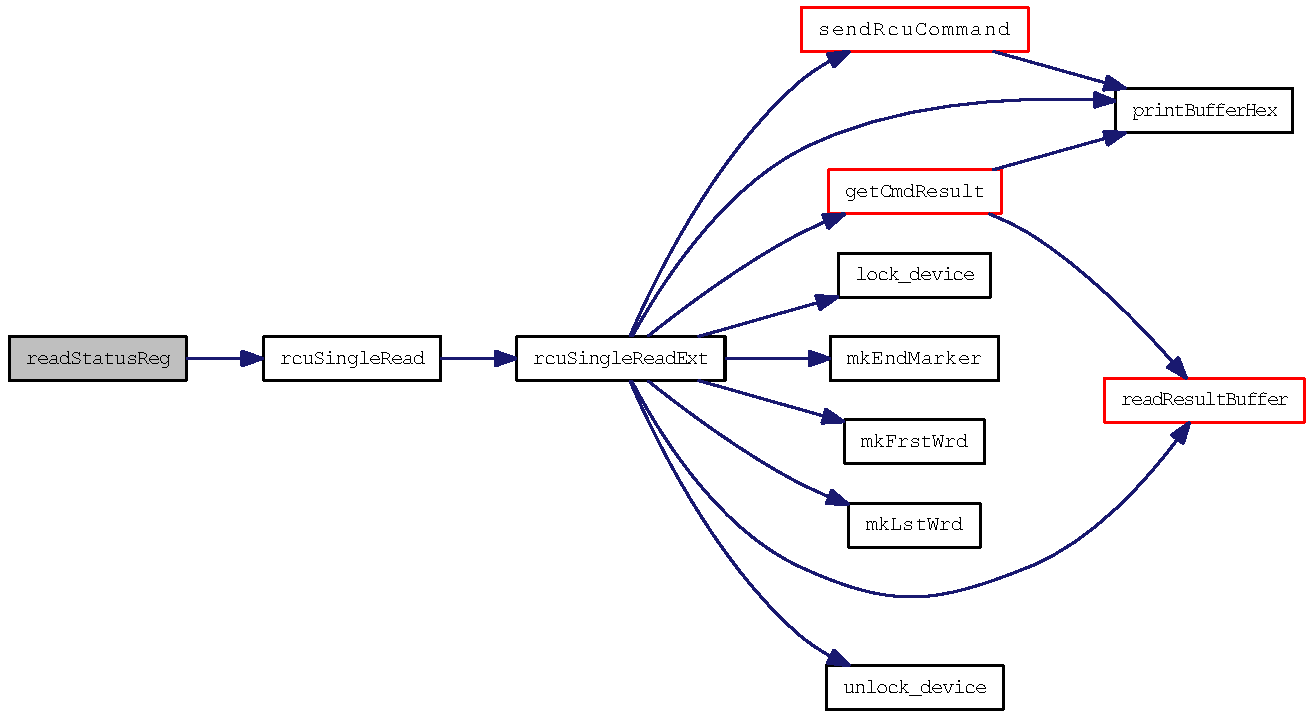
\includegraphics[width=333pt]{framever_8c_ac56165fccfc5df54af9983bef507775_cgraph}
\end{center}
\end{figure}
\hypertarget{framever_8c_6452a9d7c9fcabeb40bb5d8495300090}{
\index{framever.c@{framever.c}!step@{step}}
\index{step@{step}!framever.c@{framever.c}}
\subsubsection[step]{\setlength{\rightskip}{0pt plus 5cm}int step ()}}
\label{framever_8c_6452a9d7c9fcabeb40bb5d8495300090}


do the step-by-step frame verification 

\begin{Desc}
\item[Returns:]the errorcode \end{Desc}


Definition at line 401 of file framever.c.

References rcu\-Single\-Write().

Referenced by main().

Here is the call graph for this function:\begin{figure}[H]
\begin{center}
\leavevmode
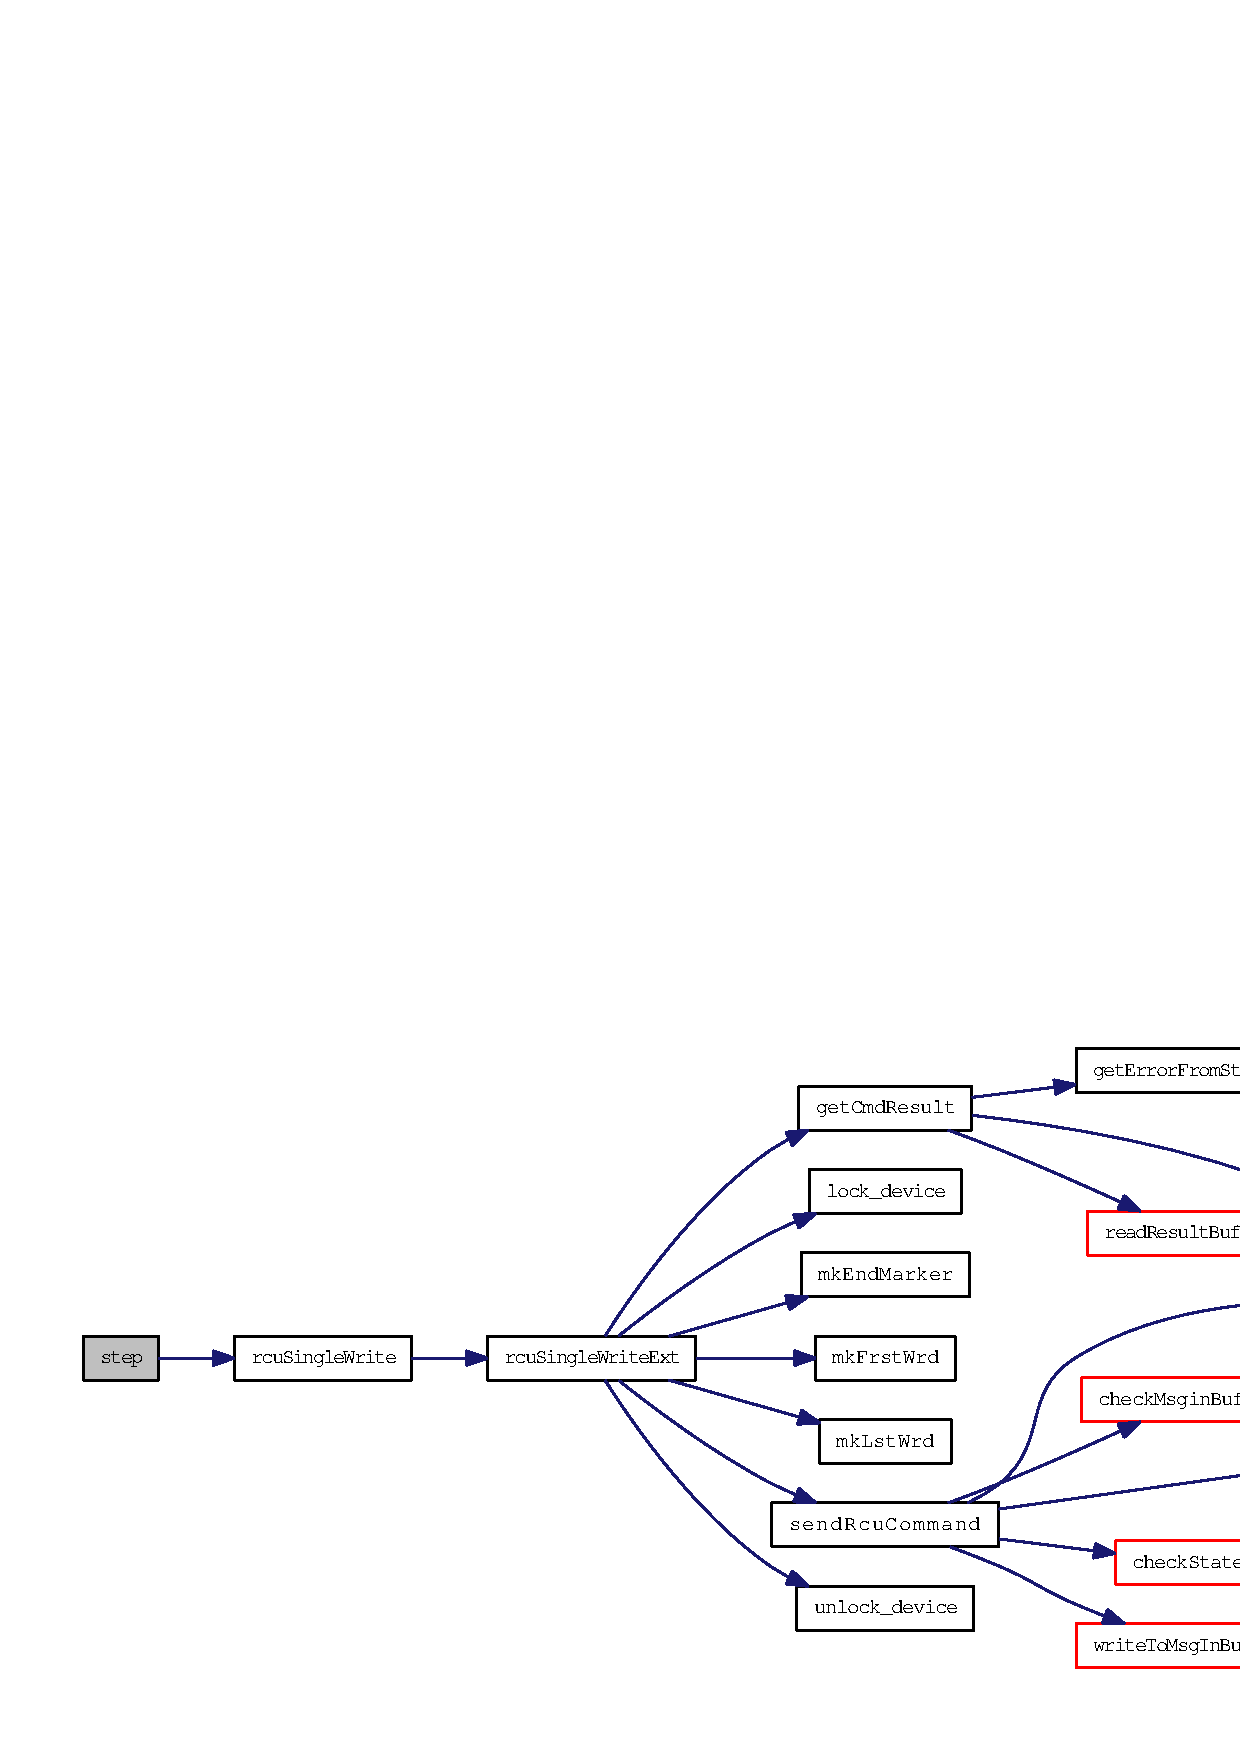
\includegraphics[width=385pt]{framever_8c_6452a9d7c9fcabeb40bb5d8495300090_cgraph}
\end{center}
\end{figure}
\hypertarget{framever_8c_5b4325e5a0e8fa3ae1c169a04e3ded7c}{
\index{framever.c@{framever.c}!writeHeaderToLogfile@{writeHeaderToLogfile}}
\index{writeHeaderToLogfile@{writeHeaderToLogfile}!framever.c@{framever.c}}
\subsubsection[writeHeaderToLogfile]{\setlength{\rightskip}{0pt plus 5cm}int write\-Header\-To\-Logfile ()}}
\label{framever_8c_5b4325e5a0e8fa3ae1c169a04e3ded7c}


Clears and opens the logfile and write a header to it, containing a timestamp. 

\begin{Desc}
\item[Returns:]not used \end{Desc}


Definition at line 520 of file framever.c.

References EXIT\_\-FAILURE.

Referenced by main().